\documentclass{standalone}
\usepackage{tikz}

\begin{document}

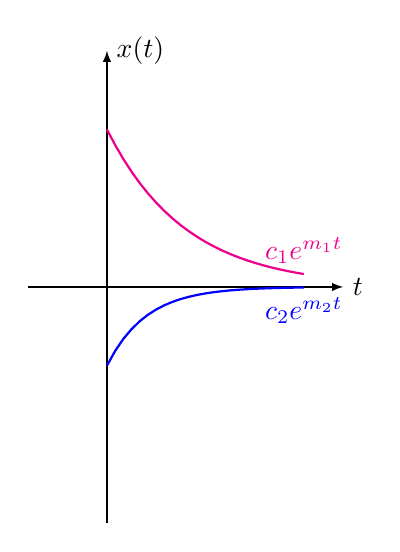
\begin{tikzpicture}[>=latex]
	\draw [->] (-1,0) -- (3,0) node [right] {\(t\)};
	\draw [->] (0,-3) -- (0,3) node [right] {\(x(t)\)};
	\draw [thick , magenta, domain=0:2.5] plot(\x , {2*exp(-\x)}) node [above] {\(c_1e^{m_1t}\)};
	\draw [thick , blue, domain=0:2.5] plot(\x , {-exp(-2*\x)}) node [below] {\(c_2e^{m_2t}\)};
\end{tikzpicture}

\end{document}
